\graphicspath{{./figures/}}
\title{virus 2}
\date{}
\usepackage{contour}
\begin{document}
\begin{frame}
    \titlepage
\end{frame}

\input{../exec-encoding/myemph-lib}

\begin{frame}{last time}
    \begin{itemize}
    \item Vienna virus code fixups
        \begin{itemize}
        \item relocation: change `data' address in appended code
        \item relocation: produce jump at beginning
        \item fixup: replace jump at beginning with normal program
        \end{itemize}
    \item real binary formats: example of ELF
        \begin{itemize}
        \item multiple segments loaded
        \item header information
        \end{itemize}
    \item virus code placement strategies
        \begin{itemize}
        \item replacing executables, temporary files
        \item appending
        \end{itemize}
    \end{itemize}
\end{frame}

\begin{frame}{scheduling note}
    \begin{itemize}
    \item no lecture Wednesday (break day)
    \item quiz due next week released by tomorrow
    \item RE assignment still due Friday
    \end{itemize}
\end{frame}


\section{viruses: where's the code?}


\begin{frame}{where to put code}
    \begin{itemize}
    \item viruses insert code in other programs
    \item Vienna's choice: end of executables
    \item search for \texttt{.COM} executables on system
    \vspace{.5cm}
    \item considerations for other options:
    \item spreading: identifying useful files to infect
        \begin{itemize}
        \item will be copied elsewhere?
        \item will be run?
        \end{itemize}
    \item stealth: avoiding detection
        \begin{itemize}
        \item Vienna: file size changes --- easy to find?
        \item Vienna: weird modification time --- easy to find?
        \end{itemize}
    \end{itemize}
\end{frame}

\begin{frame}<1>[label=whereCode]{where to put code: options}
    \begin{itemize}
    \item one \textit{or more} of:
    \item \myemph<2>{replacing executable code}
    \item \myemph<3>{after executable code (Vienna)}
    \item \myemph<4>{in unused executable code}
    \item \myemph<5>{inside OS code}
    \item \myemph<6>{in memory}
    \item \myemph<7>{replace existing code}
    \end{itemize}
\end{frame}



\subsection{appending/compressing}

\againframe<3>{whereCode}

\input{../virus/where-append}

\subsubsection{in ELF}
\usetikzlibrary{arrows.meta,patterns}

\begin{frame}[fragile,label=appendElfA]{appending to ELF file (v1)}
\begin{onlyenv}<1>
\begin{Verbatim}[fontsize=\fontsize{9}{10}\selectfont,commandchars=\\\{\}]
Program Header:
...
\colorbox{blue!40!black}{ }LOAD off    0x00000 vaddr 0x10000 paddr 0x10000 align 2**12
       filesz 0x005f8 memsz 0x005f8 flags r--
\colorbox{yellow!40!black}{ }LOAD off    0x01000 vaddr 0x11000 paddr 0x11000 align 2**12
       filesz 0x00ef5 memsz 0x00ef5 flags r-x
\colorbox{green!40!black}{ }LOAD off    0x02000 vaddr 0x12000 paddr 0x12000 align 2**12
       filesz 0x00858 memsz 0x00858 flags r--
\colorbox{orange!40!black}{ }LOAD off    0x02db8 vaddr 0x13db8 paddr 0x13db8 align 2**12
       filesz 0x00258 memsz 0x00360 flags rw-
\end{Verbatim}
\end{onlyenv}
\begin{onlyenv}<2>
\begin{Verbatim}[fontsize=\fontsize{9}{10}\selectfont,commandchars=\\\{\}]
Program Header:
...
\colorbox{blue!40!black}{ }LOAD off    0x00000 vaddr 0x10000 paddr 0x10000 align 2**12
       filesz 0x005f8 memsz 0x005f8 flags r--
\colorbox{yellow!40!black}{ }LOAD off    0x01000 vaddr 0x11000 paddr 0x11000 align 2**12
       filesz 0x00ef5 memsz 0x00ef5 flags r-x
\colorbox{green!40!black}{ }LOAD off    0x02000 vaddr 0x12000 paddr 0x12000 align 2**12
       filesz 0x00858 memsz 0x00858 flags r--
\colorbox{red}{ }LOAD off    0x02db8 vaddr 0x13db8 paddr 0x13db8 align 2**12
       filesz \sout{0x00258}\myemph{0x00860} memsz 0x00860 flags rw-
\end{Verbatim}
\end{onlyenv}
\begin{onlyenv}<3>
\begin{Verbatim}[fontsize=\fontsize{9}{10}\selectfont,commandchars=\\\{\}]
Program Header:
...
\colorbox{blue!40!black}{ }LOAD off    0x00000 vaddr 0x10000 paddr 0x10000 align 2**12
       filesz 0x005f8 memsz 0x005f8 flags r--
\colorbox{yellow!40!black}{ }LOAD off    0x01000 vaddr 0x11000 paddr 0x11000 align 2**12
       filesz 0x00ef5 memsz 0x00ef5 flags r-x
\colorbox{green!40!black}{ }LOAD off    0x02000 vaddr 0x12000 paddr 0x12000 align 2**12
       filesz 0x00858 memsz 0x00858 flags r--
\colorbox{red}{ }LOAD off    0x02db8 vaddr 0x13db8 paddr 0x13db8 align 2**12
       filesz \sout{0x00860}\myemph{0x01058} memsz \sout{0x00860}\myemph{0x01058} flags \sout{rw-}\myemph{rwx}
\end{Verbatim}
\end{onlyenv}
\begin{tikzpicture}
\draw[thick,fill=blue!40!black] (0, 0) rectangle ++(3, -.4);
\draw[thick,fill=yellow!40!black] (0, -1) rectangle ++(3, -.9);
\draw[thick,fill=green!40!black] (0, -2) rectangle ++(3, -0.5);
\draw[thick,fill=orange!40!black] (0, -2.9) rectangle ++(3, -.2);
\draw[very thick] (0, 0) rectangle (3, -3.1);
\draw[thick,-Latex] (3.1, 0) -- (3.1, -2.5);
\begin{visibleenv}<2->
    \draw[thick,pattern=north west lines] (0, -3.1) rectangle ++(3, -.5);
    \node[font=\small,anchor=west] at (3.1, -3.4) {more zeroes};
\end{visibleenv}
\begin{visibleenv}<3->
    \draw[thick,pattern=north west lines,fill=red!40!black] (0, -3.6) rectangle ++(3, -.5);
    \node[font=\small,anchor=west] at (3.1, -3.8) {virus code};
\end{visibleenv}
\begin{visibleenv}<2>
    \draw[very thick,red] (0, -2.9) rectangle ++(3,-.7);
\end{visibleenv}
\begin{visibleenv}<3>
    \draw[very thick,red] (0, -2.9) rectangle ++(3,-1.2);
\end{visibleenv}
\end{tikzpicture}
\end{frame}

\begin{frame}[fragile,label=appendElfB]{appending to ELF file (v2)}
\begin{onlyenv}<1>
\begin{Verbatim}[fontsize=\fontsize{9}{10}\selectfont,commandchars=\\\{\}]
Program Header:
...
\colorbox{blue!40!black}{ }LOAD off    0x00000 vaddr 0x10000 paddr 0x10000 align 2**12
       filesz 0x005f8 memsz 0x005f8 flags r--
\colorbox{yellow!40!black}{ }LOAD off    0x01000 vaddr 0x11000 paddr 0x11000 align 2**12
       filesz 0x00ef5 memsz 0x00ef5 flags r-x
\colorbox{green!40!black}{ }LOAD off    0x02000 vaddr 0x12000 paddr 0x12000 align 2**12
       filesz 0x00858 memsz 0x00858 flags r--
\colorbox{orange!40!black}{ }LOAD off    0x02db8 vaddr 0x13db8 paddr 0x13db8 align 2**12
       filesz 0x00258 memsz 0x00360 flags rw-
.
.
\end{Verbatim}
\end{onlyenv}
\begin{onlyenv}<2>
\begin{Verbatim}[fontsize=\fontsize{9}{10}\selectfont,commandchars=\\\{\}]
Program Header:
...
\colorbox{blue!40!black}{ }LOAD off    0x00000 vaddr 0x10000 paddr 0x10000 align 2**12
       filesz 0x005f8 memsz 0x005f8 flags r--
\colorbox{yellow!40!black}{ }LOAD off    0x01000 vaddr 0x11000 paddr 0x11000 align 2**12
       filesz 0x00ef5 memsz 0x00ef5 flags r-x
\colorbox{green!40!black}{ }LOAD off    0x02000 vaddr 0x12000 paddr 0x12000 align 2**12
       filesz 0x00858 memsz 0x00858 flags r--
\colorbox{orange!40!black}{ }LOAD off    0x02db8 vaddr 0x13db8 paddr 0x13db8 align 2**12
       filesz 0x00258 memsz 0x00360 flags rw-
\colorbox{red}{ }\myemph{LOAD off    0x04000 vaddr 0x20000 paddr 0x20000 align 2**12}
       \myemph{filesz 0x00400 memsz 0x00400 flags rwx}
\end{Verbatim}
\end{onlyenv}

\begin{tikzpicture}
\draw[thick,fill=blue!40!black] (0, 0) rectangle ++(3, -.4);
\draw[thick,fill=yellow!40!black] (0, -1) rectangle ++(3, -.9);
\draw[thick,fill=green!40!black] (0, -2) rectangle ++(3, -0.5);
\draw[thick,fill=orange!40!black] (0, -2.9) rectangle ++(3, -.2);
\begin{visibleenv}<1>
\draw[very thick] (0, 0) rectangle (3, -3.1);
\end{visibleenv}
\begin{visibleenv}<2>
\draw[very thick] (0, 0) rectangle (3, -4.25);
\end{visibleenv}
\draw[thick,-Latex] (3.1, 0) -- (3.1, -2.5);
\begin{visibleenv}<2->
    \draw[thick,pattern=north west lines,fill=red] (0, -4) rectangle ++(3, -.25);
    \node[font=\small,anchor=west] at (3.1, -4.1) {virus code};
\end{visibleenv}
\end{tikzpicture}
\end{frame}


% FIXME: work through how this work would work on ELF
\subsubsection{and compress}

\begin{frame}{compressing viruses}
    \begin{itemize}
    \item file too big? how about \myemph{compression}
    \end{itemize}
    \begin{tikzpicture}
    \draw[thick] (0, 0) rectangle (4, -6) node[midway,align=center] {original\\executable};
    \draw[line width=2mm,-Latex,black!60] (4.1, -3) -- (6.9, -3);
    \begin{scope}[xshift=7cm]
    \draw[fill=red!20,thick] (0, 0) rectangle (4, -1) node[midway] {virus code};
    \draw[fill=red!20,thick] (0, -1) rectangle (4, -2) node[midway] {decompressor};
    \draw[pattern=north west lines,pattern color=black!70,thick] (0, -2) rectangle (4, -5)
        node[midway,fill=white,align=center] {compressed \\ executable};
    \draw[fill=black!60,thick] (0, -5) rectangle (4, -6)
        node[midway,white] {unused space};
    \end{scope}
    \end{tikzpicture}
\end{frame}


\subsection{cavities}

\againframe<4>{whereCode}

\begin{frame}<1>[label=emptySpaceTypes]{other empty space}
\begin{itemize}
\item \myemph<2>{unused space between segments/sections}
\item \myemph<3>{unreachable bytes added for instruction alignment}
\item \myemph<4>{unused header space}
\item \myemph<5>{unused debugging information?}
\end{itemize}
\end{frame}



\subsubsection{gaps between segments/sections}
\begin{frame}[fragile,label=segGaps]{gaps between segments}
\begin{Verbatim}[commandchars=\\\{\}]
LOAD off    0x0000000000000000 ...
     filesz 0x00000000000036a8 ...
LOAD off    0x000000000000\myemph{4000} ...
     filesz 0x0000000000013581 ...
\end{Verbatim}
\begin{itemize}
\item first LOAD loads \texttt{0x0-0x36a8}
\item second LOAD loads \texttt{0x4000-0x17358}
    \begin{itemize}
    \item starts at \myemph{multiple of \texttt{0x1000}} b/c that's what OS can handle
    \end{itemize}
\item \texttt{0x4000-0x36a8} bytes of file not used
    \begin{itemize}
    \item<2-> (and loaded on Linux, because Linux rounds up filesz)
    \end{itemize}
\end{itemize}
\end{frame}


\subsubsection{instruction alignment}
\begin{frame}[fragile,label=lsStudy1]{unused code case study: /bin/ls}
    \begin{itemize}
    \item unreachable no-ops!
    \end{itemize}
\begin{Verbatim}[fontsize=\fontsize{9}{10}\selectfont,commandchars=Q\{\}]
...
  403788:	e9 59 0c 00 00       	jmpq   4043e6 <__sprintf_chk@plt+0x1a06>
  Qtextbf{40378d:	0f 1f 00             	nopl   (%rax)}
  403790:	ba 05 00 00 00       	mov    $0x5,%edx
...
  403ab9:	eb 4d                	jmp    403b08 <__sprintf_chk@plt+0x1128>
  Qtextbf{403abb:	0f 1f 44 00 00       	nopl   0x0(%rax,%rax,1)}
  403ac0:	4d 8b 7f 08          	mov    0x8(%r15),%r15
...
  404a01:	c3                   	retq   
  Qtextbf{404a02:	0f 1f 40 00          	nopl   0x0(%rax)}
  Qtextbf{404a06:	66 2e 0f 1f 84 00 00 	nopw   %cs:0x0(%rax,%rax,1)}
  Qtextbf{404a0d:	00 00 00 }
  404a10:	be 00 e6 61 00       	mov    $0x61e600,%esi
...
\end{Verbatim}
\end{frame}

\begin{frame}{why empty space?}
\begin{itemize}
\item Intel Optimization Reference Manual: \\
``\textbf{Assembly/Compiler Coding Rule 12. (M impact, H generality)} \\ All branch targets should be 16-byte aligned.''
\begin{itemize}
    \item better for instruction cache {\small (and TLB and related caches)}
    \item better for instruction decode logic
    \item function calls, jumps count as branches for this purpose
\end{itemize}
\end{itemize}
\end{frame}

\begin{frame}{why weird nops}
    \begin{itemize}
    \item could fill with \myemph{anything} --- unreachable
    \item {\tt nop}s allow compiler/assembler to align \myemph{without checking reachability}
    \item {\tt nop}s better for \myemph{disassembly}
        \begin{itemize}
        \item Intel manual recommends form of {\tt nop} for different lengths
        \end{itemize}
    \item possibly \myemph{better for CPU}
        \begin{itemize}
        \item ``Placing data immediately following an indirect branch
              can cause performance problems. If the data consists of all zeros,
              it looks like a long stream of ADDs to memory destinations, and this can cause
              resource conflicts\ldots''
        \end{itemize}
    \end{itemize}
\end{frame}



\subsubsection{unused header stuff}
\begin{frame}{unused header space}
    \begin{itemize}
    \item often executable metadata has empty space
    \vspace{.5cm}
    \item debugging info and info not strictly needed to run program
    \item \myemph<2>{linker allocated space for $N$ fields, used less}
    \end{itemize}
\end{frame}

\begin{frame}[label=spaceDyn,fragile]{dynamic linking cavity}
\begin{itemize}
\item Linux example from my desktop
\item {\tt .dynamic} section --- data structure used by dynamic linker:
\item format: list of 8-byte type, 8-byte value
    \begin{itemize}
    \item terminated by type == 0 entry
    \end{itemize}
\end{itemize}
\begin{Verbatim}[fontsize=\fontsize{9}{10}\selectfont,commandchars=Q\{\}]
Contents of section .dynamic:
 600e28 01000000 00000000 01000000 00000000  ................
    Qtextit{... several non-empty entries ...}
 600f88 f0ffff6f 00000000 56034000 00000000  ...o....V.@.....
    Qtextit{VERSYM (required library version info at) 0x400356}
 600f98 Qtextit{00000000 00000000 00000000 00000000}  ................
    Qtextit{NULL --- end of linker info}
 600fa8 Qtextbf{00000000 00000000 00000000 00000000}  ................
    Qtextit{unused! (and below)}
 600fb8 Qtextbf{00000000 00000000 00000000 00000000}  ................
 600fc8 Qtextbf{00000000 00000000 00000000 00000000}  ................
 600fd8 Qtextbf{00000000 00000000 00000000 00000000}  ................
 600fe8 Qtextbf{00000000 00000000 00000000 00000000}  ................
\end{Verbatim}
\end{frame}




\subsubsection{exercise: cavity finding ease}
\input{../virus/cavity-finding-ex}

\subsubsection{chaining cavaties (CIH case study)}
\usetikzlibrary{arrows.meta,patterns}

\begin{frame}{is there enough empty space?}
\begin{itemize}
    \item cavities look awfully small
    \item really small viruses?
    \item solution: chain cavities tgoether
\end{itemize}
\end{frame}

\begin{frame}{case study: CIH (1)}
    \begin{tikzpicture}
    \draw[thick] (0, 0) rectangle (4, -6) node[midway,align=center] {original\\executable};
    \draw[line width=2mm,-Latex,black!60] (4.1, -3) -- (6.9, -3);
    \begin{scope}[xshift=7cm]
    \draw[fill=red!20,thick] (0, 0) rectangle (4, -0.5) node[midway] {virus startup code};
    \draw[fill=red!20,thick] (0, -0.5) rectangle (4, -1) node[midway] {virus code locs};
    \draw[thick] (0, -1) rectangle (4, -6);
    \draw[fill=red!20,thick] (0, -3) rectangle (4, -3.5)
        node[midway] {virus code part 1};
    \draw[fill=red!20,thick] (0, -4) rectangle (4, -4.5)
        node[midway] {virus code part 2};
    \draw[fill=red!20,thick] (0, -5) rectangle (4, -5.5)
        node[midway] {virus code part 3};
    \draw[dashed,thin,-Latex] (4, -0.75) -- (4.5, -0.75) |- (4, -3.25);
    \draw[dashed,thin,-Latex] (4, -0.75) -- (4.5, -0.75) |- (4, -4.25);
    \draw[dashed,thin,-Latex] (4, -0.75) -- (4.5, -0.75) |- (4, -5.25);
    \end{scope}
    \end{tikzpicture}
\end{frame}

\begin{frame}{case study: CIH (2)}
    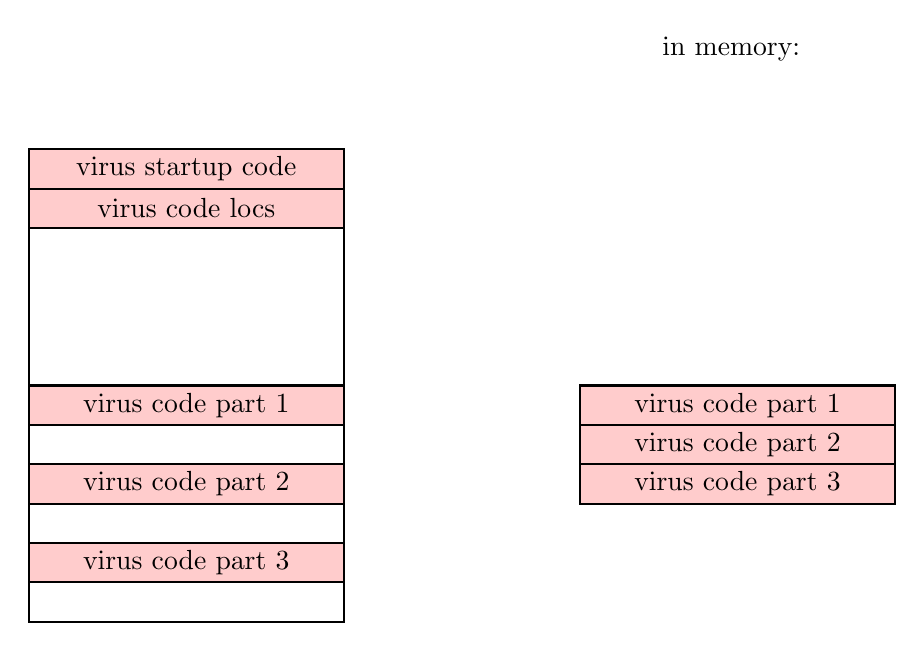
\begin{tikzpicture}
    \draw[fill=red!20,thick] (0, 0) rectangle (4, -0.5) node[midway] {virus startup code};
    \draw[fill=red!20,thick] (0, -0.5) rectangle (4, -1) node[midway] {virus code locs};
    \draw[thick] (0, -1) rectangle (4, -6);
    \draw[fill=red!20,thick] (0, -3) rectangle (4, -3.5)
        node[midway] {virus code part 1};
    \draw[fill=red!20,thick] (0, -4) rectangle (4, -4.5)
        node[midway] {virus code part 2};
    \draw[fill=red!20,thick] (0, -5) rectangle (4, -5.5)
        node[midway] {virus code part 3};
    \begin{scope}[xshift=7cm]
        \node[align=center,anchor=south] at (2, 1) { in memory: };
        \draw[fill=red!20,thick] (0, -3) rectangle (4, -3.5)
            node[midway] {virus code part 1};
        \draw[fill=red!20,thick] (0, -3.5) rectangle (4, -4)
            node[midway] {virus code part 2};
        \draw[fill=red!20,thick] (0, -4) rectangle (4, -4.5)
            node[midway] {virus code part 3};
    \end{scope}
    \end{tikzpicture}
\end{frame}

\begin{frame}{CIH cavities}
    \begin{itemize}
    \item gaps between sections
        \begin{itemize}
        \item common Windows linker aligned sections
        \item (align = start on address multiple of $N$, e.g. $4096$)
        \end{itemize}
    \item reassembling code avoids worrying about splitting instructions
    \end{itemize}
\end{frame}



\section{discussion: detecting cavity hiding}
\begin{frame}{detecting cavity hiding?}
    \begin{itemize}
    \item thought for future: detecting cavity hiding?
    \vspace{.5cm}
    \item example: filling empty space in header --- what should we look for?
        \begin{itemize}
        \item<2-> stuff that looks like machine code?
        \item<2-> validate matches executable data structure?
        \end{itemize}
    \vspace{.5cm}
    \item<3-> follow-up: possibility for false positives?
        \begin{itemize}
        \item<4-> additional executable format features?
        \item<4-> values that happen to be same as machine code?
        \end{itemize}
    \end{itemize}
\end{frame}


\subsection{boot sector and BIOS/UEFI}
\againframe<5>{whereCode}
\usetikzlibrary{arrows.meta,chains}

\begin{frame}<1-2>[fragile,label=bootProc]{boot process}
    \pdftooltip{
    \begin{tikzpicture}
        \begin{scope}[start chain=going below,every node/.style={draw,align=center,join,on chain,thick,minimum width=3.5cm},
                      every join/.style={-Latex,thick}]
        \node[draw=none] (fixedLoc) { processor reset };
        \node[alt=<3>{draw=orange,very thick}{}] (bios) {BIOS/EFI \\ \small (chip on motherboard)};
        \node[alt=<2>{draw=orange,very thick}{}] (bootloader) {bootloader};
        \node[alt=<4>{draw=orange,very thick}{}] (os) {operating system};
        \end{scope}
        \node[left=.5cm of bios,font=\small] (biosLabel) {very CPU/motherboard-specific code};
        \draw[-Latex,thick] (biosLabel) -- (bios);
        \node[left=.5cm of bootloader,font=\small,align=right] (bootloaderLabel) {fixed location on disk \\ code that understands files};
        \draw[-Latex,thick] (bootloaderLabel) -- (bootloader);
        \node[left=.5cm of os,font=\small] (osLabel) {files in a filesystem};
        \draw[-Latex,thick] (osLabel) -- (os);
    \end{tikzpicture}
    }{
        Boot process, starting from processor reset.
        First, the BIOS of EFI is loadeed from a chip on the motherboard. 
        Then, a bootloader in a fixed location on disk runs, which has the code to figure out
        where individual files are on disk. This finally loads the operating system code
        from its files.
    }
\end{frame}

\begin{frame}{bootloaders in the DOS era}
    \begin{itemize}
    \item used to be common to boot from floppies
    \item \myemph{default to booting from floppy} if present
        \begin{itemize}
        \item even if hard drive to boot from
        \end{itemize}
    \item applications distributed as bootable floppies
    \item so bootloaders on all devices were a target for viruses
    \end{itemize}
\end{frame}

\begin{frame}{historic bootloader layout}
    \begin{itemize}
    \item bootloader in \myemph{first sector} (512 bytes) of device
    \item (along with partition information)
    \item code in BIOS to copy bootloader into RAM, start running
    \item bootloader responsible for disk I/O etc.
        \begin{itemize}
        \item some library-like functionality in BIOS for I/O
        \end{itemize}
    \end{itemize}
\end{frame}

\begin{frame}[fragile]{bootloader viruses}
    \newcommand{\tearBox}{
        \draw[very thick] (0, -6) -- (0, 0) -- (4, 0) -- (4, -6);
        \draw[thick] (0, -6) -- (1.2, -5.5) -- (2., -6.6) -- (2.6, -5.8) -- (3.5, -6.6) -- (4, -6);
    }
    \begin{itemize}
    \item example: Stoned
    \end{itemize}
    \pdftooltip{
    \begin{tikzpicture}
        \draw[fill=green!20] (0, 0) rectangle (4, -.2);
        \draw[fill=yellow!20] (0, -.2) rectangle (4, -0.5) node[midway,font=\tiny] { partition table };
        \draw[fill=green!20] (0, -.5) rectangle (4, -1.0) node[midway,font=\small] { bootloader };
        \tearBox
        \begin{scope}[xshift=7cm]
        \draw[fill=violet!20] (0, 0) rectangle (4, -.2);
        \draw[fill=yellow!20] (0, -.2) rectangle (4, -0.5) node[midway,font=\tiny] { partition table };
        \draw[fill=violet!20] (0, -.5) rectangle (4, -1.0) node[midway,font=\small] { virus code };
        \begin{scope}[yshift=-4cm]
        \draw[fill=green!20] (0, 0) rectangle (4, -.2);
        \draw[fill=green!20] (0, -.5) rectangle (4, -1.0) node[midway,font=\small] { saved bootloader };
        \draw[dashed,fill=yellow!20] (0, -.2) rectangle (4, -0.5) node[midway,font=\tiny] { partition table (unused) };
        \end{scope}
        \tearBox 
        \end{scope}
        \draw[line width=1mm,black!50, -Latex] (4.2, -3) -- (6.8, -3);
        %
        \begin{pgfonlayer}{bg}
            \begin{visibleenv}<2>
                \path[fill=blue!30] (0, -4) rectangle (4, -5) node[midway] { data here??? };
            \end{visibleenv}
        \end{pgfonlayer}
    \end{tikzpicture}
    }{
        The original contents of disk shows a bootloader at the beginning with a partition table
        in the middle of it.
        This is transformed to the bootloader being replaced by the virus code (but the partition table
        is preserved). So the virus can
        run the original bootloader after it finishes, a copy of the original bootloader is saved
        elsewhere on disk
    }
\end{frame}

\begin{frame}{data here???}
    \begin{itemize}
        \item might be data there --- risk
        \item some unused space after partition table/boot loader common
            \begin{itemize}
            \item (allegedly)
            \end{itemize}
        \item also be filesystem metadata not used on smaller floppies/disks
        \vspace{.5cm}
        \item but could be wrong --- oops
    \end{itemize}
\end{frame}

\begin{frame}{modern bootloaders --- UEFI}
    \begin{itemize}
    \item BIOS-based boot is going away (slowly)
    \item new thing: UEFI (Universal Extensible Firmware Interface)
    \item like BIOS:
        \begin{itemize}
        \item library functionality for bootloaders
        \item loads initial code from disk/DVD/etc.
        \end{itemize}
    \item unlike BIOS:
        \begin{itemize}
        \item much more understanding of file systems
        \item much more modern set of library calls
        \end{itemize}
    \end{itemize}
\end{frame}

\againframe<3>{bootProc}

\begin{frame}{BIOS/UEFI implants}
    \begin{itemize}
    \item infrequent
    \item BIOS/UEFI code is \myemph{very non-portable}
    \item BIOS/UEFI update may require physical access
    \item BIOS/UEFI code may require cryptographic signatures
    \item \ldots but \myemph{very hard to remove} --- ``persist'' other malware
    \item reports of BIOS/UEFI-infecting ``implants''
        \begin{itemize}
        \item sold by Hacking Team (Milan-based malware company) 
        \item listed in leaked NSA Tailored Access Group catalog
        \end{itemize}
    \end{itemize}
\end{frame}

\againframe<4>{bootProc}

\begin{frame}{system files}
    \begin{itemize}
    \item simpliest strategy: stuff that runs when you start your computer
    \item add a new startup program, run in the background
        \begin{itemize}
        \item easy to blend in
        \end{itemize}
    \vspace{.5cm}
    \item alternatively, infect one of many system programs automatically run
    \end{itemize}

    % FIXME: example from CodeRed or similar?
\end{frame}



\subsection{memory residence}
\againframe<6>{whereCode}

\begin{frame}{memory residence}
    \begin{itemize}
    \item malware wants to keep doing stuff
    \item one option --- background process (easy on modern OSs)
    \item also stealthy options:
        \begin{itemize}
        \item insert self into OS code
        \item insert self into other running programs
        \end{itemize}
    \end{itemize}
\end{frame}
 % FIXME: should have more extensive discussion of this somewhere

\subsection{replacing existing code}
\againframe<7>{whereCode}

\subsection{(if time) exercise: easiest to find?}
\begin{frame}{virus: easiest code to find?}
    \begin{itemize}
    \item what should be easiest/hardest to identify \\
        without many false positives?
    \vspace{.5cm}
        \item A. replaced executable
        \item B. appended to executable w/o compression
        \item C. replaced cavities
        \item D. replaced bootloader
        \item E. new automatically started system program
    \end{itemize}
\end{frame}

\begin{frame}{virus: easiest code to find pro/con}
    \begin{itemize}
    \item A. replaced executable
        \begin{itemize}
        \item + executable size size change
        \item + could detect write+launch executable
        \item - programs running programs is common (e.g. start browser)
        \item - confused with software updater
        \end{itemize}
    \item B. appended to executable w/o compression
        \begin{itemize}
        \item + executable size change
        \item + unusual segment/section layout
        \item - confused with unusual compilers
        \end{itemize}
    \item C. replaced cavities
        \begin{itemize}
        \item + code outside of segments/sections if virus not careful
        \item + machine code patterns not seen by compilers
        \item - need to search entire exe file
        \item - confused with unusual compilers?
        \end{itemize}
    \item D. replaced bootloader
        \begin{itemize}
        \item + can check versus normal for OS
        \item - need to handle new OS versions, etc.
        \end{itemize}
    \item E. new automatically started system program
        \begin{itemize}
        \item + can check versus normal list for OS
        \item - need to handle new OS versions
        \item - lots of legitimate programs may run at startup
        \end{itemize}
    \end{itemize}
\end{frame}


\section{virus: getting code invoked}

\begin{frame}<1-2>[label=invokeOptions]{invoking virus code: options}
    \begin{itemize}
    \item boot loader
    \item \myemph<2>{change starting location} 
    \item alternative approaches: ``entry point obscuring''
    \item \myemph<3>{edit code that's going to run anyways}
    \item \myemph<4>{replace a function pointer} (or similar)
    \item \ldots
    \end{itemize}
\end{frame}


\subsection{changing start location}

\begin{frame}[fragile,label=invokeStarting]{starting locations}
\begin{Verbatim}[fontsize=\fontsize{10}{11}\selectfont,commandchars=Q\{\}]
/bin/ls:     file format elf64-x86-64
/bin/ls
architecture: i386:x86-64, flags 0x00000112:
EXEC_P, HAS_SYMS, D_PAGED
start address Qmyemph{0x00000000004049a0}
\end{Verbatim}
    \begin{itemize}
    \item modern executable formats have `starting address' field
    \item just change it, insert jump to old address after virus code
    \end{itemize}
\end{frame}




\subsection{overwrite existing code}
\begin{frame}<1>[fragile,label=runAnyways]{run anyways?}
    \begin{itemize}
    \item add code at start of program (Vienna)
        \begin{itemize}
        \item \myemph<2>{plus restore replaced code after running malware code}
        \end{itemize}
    \item return with padding after it:
\begin{Verbatim}[fontsize=\fontsize{10}{11}\selectfont,commandchars=Q\{\}]
  404a01:       c3                      Qtextbf{retq}
  404a02:       0f 1f 40 00             nopl   0x0(%rax)
                Qtextit{replace with}
  404a01:       e9 XX XX XX XX          Qtextbf{jmpq    YYYYYYY}
\end{Verbatim}
        \begin{itemize}
        \item plus return after running malware code
        \end{itemize}
    \item any random place in program?
        \begin{itemize}
        \item just not in the \myemph{middle of instruction}
        \item and \myemph<2>{replace orignal code after running malware code}
        \end{itemize}
    \end{itemize}
\end{frame}

\begin{frame}[fragile,label=findValidChallenge]{challenge: valid locations}
    \begin{itemize}
    \item x86: probably don't want a full instruction parser
    \item x86: might be non-instruction stuff mixed in with code:
\begin{lstlisting}[language=myasm,style=smaller]
do_some_floating_point_stuff:
            movss float_one(%rip), %xmm0
            ...
            retq
float_one: .float 1
\end{lstlisting}
    \begin{itemize}
        \item floating point value one ({\tt 00 00 80 3f}) is not valid machine code
        \item disassembler might lose track of instruction boundaries
    \end{itemize}
    \end{itemize}
\end{frame}

\begin{frame}[fragile,label=findValidFindFunc]{finding function calls}
    \begin{itemize}
    \item one idea: replace calls
    \item normal x86 call FOO: {\tt E8 \textit{(32-bit value: PC - address of foo)}}
    \item could look for E8 in code --- \myemph{lots of false positives}
        \begin{itemize}
        \item probably even if one excludes out-of-range addresses
        \end{itemize}
    \end{itemize}
\end{frame}

\begin{frame}[fragile,label=findValidFindFunc2]{really finding function calls}
\lstset{language=myasm,style=small}
    \begin{itemize}
    \item e.g. some popular compilers started x86-32 functions with
\begin{lstlisting}
foo:
    push %ebp       // push old frame pointer
    // 0x55
    mov %esp, %ebp  // set frame pointer to stack pointer
    // 0x89 0xec
\end{lstlisting}
    \item use to identify when {\tt e8} refers to real function
    \begin{itemize}
    \item (full version: also have some other function start patterns)
    \end{itemize}
    \end{itemize}
\end{frame}

\againframe<2>{runAnyways}

\begin{frame}{restoring replaced code?}
    \begin{itemize}
    \item Vienna: just write to memory addres
    \vspace{.5cm}
    \item modern OS: segfault/general protection fault
        \begin{itemize}
        \item code loaded read-only
        \end{itemize}
    \item easy solution: make library call to make it writable
        \begin{itemize}
        \item Linux: \texttt{mprotect}
        \item functionality exists to, e.g., allow compiling code at runtime
        \end{itemize}
    \end{itemize}
\end{frame}


\section{dynamic linking}
    % FIXME: shorten linking intro

\begin{frame}{linking}
    \begin{tikzpicture}
    \node[draw,font=\tt,very thick] (theCall) {callq printf};
    \node[draw,font=\tt,below=5cm of theCall,very thick] (theCallResolved) {callq 0x458F0};
    \draw[very thick,-Latex] (theCall) -- (theCallResolved);
    \end{tikzpicture}
\end{frame}

\begin{frame}{static v. dynamic linking}
    \begin{itemize}
    \item static linking --- linking \myemph{to create executable}
    \item dynamic linking --- linking \myemph{when executable is run}
    \vspace{.5cm}
    \item<2> conceptually: no difference in how they work
    \item<2> reality --- very different mechanisms
        \begin{itemize}
        \item extra indirection to avoid modifying much code at runtime
        \item change \textit{lookup table} instead of code for library locations
        \end{itemize}
    \end{itemize}
\end{frame}


\subsection{aside: strace, statically linked strace}
\begin{frame}{interlude: strace}
\begin{itemize}
\item {\tt strace} --- system call tracer
    \begin{itemize}
    \item on Linux, some other Unices
    \item OS X approx. equivalent: {\tt dtruss}
    \item Windows approx. equivalent: Process Monitor
    \end{itemize}
\item indicates what system calls (operating system services) used by a program
\end{itemize}
\end{frame}

\begin{frame}[fragile,label=staticStrace]{statically linked hello.exe}
\begin{itemize}
\item \small{\tt gcc -no-pie -static -o hello-static.exe hello.s}
\item \small{\tt strace ./hello-static.exe}:
\end{itemize}
\begin{Verbatim}[commandchars=@\{\},fontsize=\fontsize{8}{9}\selectfont]
execve("./hello-static.exe", ["./hello-static.exe"], [/* 46 vars */]) = 0
@myemphTwo{uname({sysname="Linux", nodename="reiss-lenovo", ...}) = 0}
@myemphTwo{brk(NULL)                               = 0x20a5000}
@myemphThree{brk(0x20a61c0)                          = 0x20a61c0}
@myemphTwo{arch_prctl(ARCH_SET_FS, 0x20a5880)      = 0}
@myemphTwo{readlink("/proc/self/exe", "/home/cr4bd/spring2017/cs4630/sl"..., 4096) = 62}
@myemphThree{brk(0x20c71c0)                          = 0x20c71c0}
@myemphThree{brk(0x20c8000)                          = 0x20c8000}
@myemphTwo{access("/etc/ld.so.nohwcap", F_OK)}      = -1 ENOENT (No such file or directory)
@myemphFour{fstat(1, {st_mode=S_IFCHR|0620, st_rdev=makedev(136, 1), ...}) = 0}
@myemphFour{write(1, "Hello, World!\n", 14)         = 14}
@myemphFive{exit_group(14)}                          = ?
+++ exited with 14 +++
\end{Verbatim}
\begin{tikzpicture}[overlay,remember picture]
    \tikzset{
        overBoxGeneric/.style={
            anchor=center,
            align=center,
            draw,
            rectangle,
            fill=white,
            draw=red!70!black,very thick},
        overBox/.style={
            overBoxGeneric,
            at=(boxLoc),
        },
        overBoxB/.style={
            overBoxGeneric,
            at=(boxLocB),
        },
    }
    \coordinate (boxLoc) at ([yshift=-3.5cm]current page.center);
    \begin{visibleenv}<2>
        \node[overBox] {
            standard library startup
        };
    \end{visibleenv}
    \begin{visibleenv}<3>
        \node[overBox] {
            memory allocation
        };
    \end{visibleenv}
    \begin{visibleenv}<4>
        \node[overBox] {
            implementation of puts
        };
    \end{visibleenv}
    \begin{visibleenv}<5>
        \node[overBox] {
            standard library shutdown
        };
    \end{visibleenv}
\end{tikzpicture}
\end{frame}



\subsection{example: strace hello.exe dynamic}

\begin{frame}[fragile,label=straceDynamic]{dynamically linked hello.exe}
\begin{itemize}
\item \small{\tt gcc -no-pie -o hello.exe hello.s}
\item \small{\tt strace ./hello.exe}:
\end{itemize}
\begin{Verbatim}[commandchars=@\{\},fontsize=\fontsize{8}{9}\selectfont]
execve("./hello.exe", ["./hello.exe"], [/* 46 vars */]) = 0
@textit{...}
@myemphThree{mmap(NULL, 8192, PROT_READ|PROT_WRITE, MAP_PRIVATE|MAP_ANONYMOUS, -1, 0)} = 0x7fdfeeb39000
access("/etc/ld.so.preload", R_OK)      = -1 ENOENT (No such file or directory)
open("/etc/ld.so.cache", O_RDONLY|O_CLOEXEC) = 3
fstat(3, {st_mode=S_IFREG|0644, st_size=137808, ...}) = 0
@textit{...}
open("@myemphTwoB{/lib/x86_64-linux-gnu/libc.so.6}", O_RDONLY|O_CLOEXEC) = 3
@myemphFour{read(3, "\177ELF\2\1\1\3\0\0\0\0\0\0\0\0\3\0>\0\1\0\0\0P\t\2\0\0\0\0\0"..., 832) = 832}
fstat(3, {st_mode=S_IFREG|0755, st_size=1864888, ...}) = 0
@myemphFive{mmap(NULL, 3967392, PROT_READ|PROT_EXEC, ..., 3, 0) = 0x7fdfee54d000}
mprotect(0x7fdfee70c000, 2097152, PROT_NONE) = 0
@myemphFive{mmap(0x7fdfee90c000, 24576, PROT_READ|PROT_WRITE, ..., 3, 0x1bf000) = 0x7fdfee90c000}
@myemphSix{mmap(0x7fdfee912000, 14752, PROT_READ|PROT_WRITE, ..., -1, 0) = 0x7fdfee912000}
close(3)                                = 0
@textit{...}
write(1, "Hello, World!\n", 14)         = 14
exit_group(14)                          = ?
+++ exited with 14 +++
\end{Verbatim}
\begin{tikzpicture}[overlay,remember picture]
    \tikzset{overBox/.style={at=(boxLoc),anchor=center,align=center,draw,rectangle,fill=white,draw=red!70!black,very thick}}
    \coordinate (boxLoc) at ([yshift=-2cm]current page.center);
    \begin{visibleenv}<2>
        \node[overBox] {
            the standard C library (includes {\texttt{puts}})
        };
    \end{visibleenv}
    \begin{visibleenv}<3>
        \node[overBox] {
            memory allocation (different method)
        };
    \end{visibleenv}
    \begin{visibleenv}<4>
        \node[overBox] {
            read standard C library header
        };
    \end{visibleenv}
    \begin{visibleenv}<5>
        \node[overBox] {
            load standard C library ({\tt 3} = opened file)
        };
    \end{visibleenv}
    \begin{visibleenv}<6>
        \node[overBox] {
            allocate zero-initialized data segment for C library
        };
    \end{visibleenv}
\end{tikzpicture}
\end{frame}



\subsection{where's the linker}

\begin{frame}{where's the linker}
\begin{itemize}
    \item Where's the code that calls {\tt open("...libc.so.6")}?
    \item Could check {\tt hello.exe} --- it's not there!
    \vspace{.5cm}
    \item<2> instead: ``interpreter'' {\tt /lib64/ld-linux-x86-64.so.2}
    \item<2> on Linux: contains loading code instead of core OS
        \begin{itemize}
        \item OS loads it instead of program
        \end{itemize}
\end{itemize}
\end{frame}

\begin{frame}[fragile,label=interpObjdump]{objdump --- the interpreter}
\begin{itemize}
\item excerpt from {\tt objdump -sx hello.exe}:
\end{itemize}
\begin{Verbatim}[commandchars=@\{\},fontsize=\fontsize{8}{9}\selectfont]
Program Header:
@textit{...}
  INTERP off    0x0000238 vaddr 0x0@myemph{400318} paddr 0x0400238 align 2**0
         filesz 0x000001c memsz 0x000001c flags r--
@textit{...}
Contents of section .interp:
 @myemph{400318} 2f6c6962 36342f6c 642d6c69 6e75782d  @myemph{/lib64/ld-linux-}
 400328 7838362d 36342e73 6f2e3200           @myemph{x86-64.so.2}.    
\end{Verbatim}
\end{frame}


\subsection{knowing what to load?}
\begin{frame}[fragile,label=dynLinkNeeded1]{dynamic linking: what to load? (1)}
\begin{itemize}
\item excerpt from {\tt objdump -sx hello.exe}:
\end{itemize}
\begin{Verbatim}[commandchars=@\{\},fontsize=\fontsize{9}{10}\selectfont]
Program Header:
@textit{...}
 @myemph{DYNAMIC} off    0x0000000000002e20 vaddr 0x0000000000403e20 paddr 0x0000000000403e20 align 2**3
         filesz 0x00000000000001d0 memsz 0x00000000000001d0 flags rw-
@textit{...}
Dynamic Section:
  @myemph{NEEDED               libc.so.6}
  INIT                 0x0000000000401000
  ...
  STRTAB               0x0000000000400420
  ...
\end{Verbatim}
\begin{itemize}
\item program header: identifies where dynamic linking info is
\item dynamic linking info: array of key-value pairs
    \begin{itemize}
    \item needed libraries
    \item constructor locations (`INIT')
    \item string table location
    \item \ldots
    \end{itemize}
\end{itemize}
\end{frame}



\section{backup slides}
\begin{frame}{backup slides}
\end{frame}

\subsection{needed info encoding}

\providecommand{\myemphA}[1]{\myemph<1>{#1}}
\providecommand{\myemphB}[1]{\myemph<2>{#1}}
\providecommand{\myemphAB}[1]{\myemph<1-2>{#1}}
\providecommand{\myemphC}[1]{\myemph<3>{#1}}
\begin{frame}[fragile,label=dynLinkNeeded2]{dynamic linking: what to load? (2)}
\begin{itemize}
\item excerpt from {\tt objdump -sx hello.exe}:
\end{itemize}
\begin{Verbatim}[commandchars=@\{\},fontsize=\fontsize{9}{10}\selectfont]
Program Header:
@textit{...}
 DYNAMIC off    0x0000000000002e20 vaddr @myemph{0x0000000000403e20} paddr 0x0000000000403e20 align 2**3
         filesz 0x00000000000001d0 memsz 0x00000000000001d0 flags rw-
@textit{...}
Dynamic Section:
  @myemphAB{NEEDED               libc.so.6}
  @myemphC{INIT                 0x0000000000401000}
  ...
  @myemphB{STRTAB}               0x0000000000400420
  ...
@textit{...}
 @myemphAB{403e20} @myemphA{01000000 00000000} @myemphB{01000000 00000000}  ................
 403e30 @myemphC{0c000000 00000000 00104000 00000000}  ..........@.....
\end{Verbatim}
\hrule
type \myemphA{0x1 = ``DT\_NEEDED''} (from ELF manual)\\
value \myemphB{0x1 = string table entry 1} \\
\hrule
type \myemphC{0xC = ``DT\_INIT''} \\
value \myemphC{0x401000} \\
\end{frame}


\subsection{ELF LOAD}
\usetikzlibrary{arrows.meta,decorations.pathmorphing,patterns}

\begin{frame}<2->{ELF LOAD}
\begin{tikzpicture}
\begin{pgfonlayer}{fg}
    \draw[very thick] (0, 0) rectangle (4, 6);
\node[font=\huge,black!25,align=center] at (2, 3) {
    program \\ on\\ disk
};
\end{pgfonlayer}
\coordinate (header tl) at (4, 0.5);
\coordinate (header br) at (0, 0);
\coordinate (load off) at (0, 1);
\coordinate (load end) at (0, 2.54);
\draw[thick,Latex-,font=\small] (0, 0) -- ++(-.5, 0) node[left,align=right] {off {\tt 0}\\ (start)};

\begin{scope}[xshift=6cm]
    \begin{pgfonlayer}{fg}
        \draw[very thick] (0, 7) -- (0, 0) -- (4, 0) -- (4, 7);
        \draw[overlay,very thick,decorate,decoration={zigzag,segment length=2.5mm}] (0, 7) -- (4, 7);
    \node[font=\huge,black!25,align=center] at (2, 3) {
        program \\ in\\ memory
    };
    \end{pgfonlayer}
    \coordinate (vaddr off) at (4, 4);
    \coordinate (vaddr end copy) at (4, 5.54);
    \coordinate (vaddr end all) at (4, 6.64);
\draw[thick,Latex-,font=\small] (4, 0) -- ++(.5, 0) node[right,align=left] {addr {\tt 0}};
\end{scope}
\begin{visibleenv}<2->
    \fill[blue!30] (header tl) rectangle (header br);
    \node[align=left,font=\small\tt,anchor=north west,draw] (load) at (1, -.25) {
        LOAD off {\color{green!50!black}0x1000} vaddr {\color{violet!70}0x4000} \ldots \\
        \hspace{1cm} filesz 0x1544 memsz 0x2644 \ldots
    };
    \draw[dotted,thick] ([yshift=-1mm]header tl -| header br) -- (load.north west);
    \draw[dotted,thick] ([xshift=3cm,yshift=-1mm]header tl -| header br) -- (load.north east);
\end{visibleenv}
\begin{visibleenv}<3->
    \draw[very thick,Latex-] (load off) -- ++(-.5cm,0) node[left,font=\small] {{\color{green!50!black}\tt 0x1000}};
    \draw[very thick,Latex-] (vaddr off) -- ++ (.5cm, 0) node[right,font=\small] {{\color{violet!70}\tt 0x4000}};
    \draw[thick,Latex-Latex] ([xshift=-.15cm]load off) -- ([xshift=-.15cm]load end)
        node[midway,font=\small,left] {\tt 0x1544};
    \draw[thick,Latex-Latex] ([xshift=.15cm]vaddr off) -- ([xshift=.15cm]vaddr end copy)
        node[midway,font=\small,right] {\tt 0x1544};
    \draw[thick,Latex-Latex] ([xshift=-4.15cm]vaddr off) -- ([xshift=-4.15cm]vaddr end all)
        node[midway,font=\small,left] {\tt 0x2644};
    \fill[red!20] (load off) rectangle ([xshift=4cm]load end);
    \fill[red!20] (vaddr off) rectangle ([xshift=-4cm]vaddr end copy);
    \fill[pattern=north west lines] (vaddr end copy) rectangle ([xshift=-4cm]vaddr end all);
\end{visibleenv}
\end{tikzpicture}
\end{frame}


\subsection{static symbol/relocation tables}
\begin{frame}[fragile,label=linkingExAsm]{hello.s}
\begin{lstlisting}
.data
string: .asciz "Hello, World!"
.text
.globl main
main:
    movq $string, %rdi
    call puts
    ret
\end{lstlisting}
\end{frame}

\begin{frame}[fragile,label=linkingExObjRepeat]{hello.o (pre-static or dynamic linking)}
\begin{Verbatim}[commandchars=\\\{\},fontsize=\fontsize{9}{10}\selectfont]
SYMBOL TABLE:
0000000000000000 l    d  .text  0000000000000000 .text
0000000000000000 l    d  .data  0000000000000000 .data
0000000000000000 l    d  .bss   0000000000000000 .bss
0000000000000000 l       .data  0000000000000000 string
0000000000000000 \myemphSix{g}       \myemphSeven{.text  0000000000000000} main
0000000000000000         \myemphTwo{*UND*  0000000000000000 puts}

RELOCATION RECORDS FOR [.text]:
OFFSET           TYPE              VALUE 
0000000000000003 \myemphFive{R_X86_64_32S}      \myemphFour{.data}
0000000000000008 \myemphFive{R_X86_64_PC32}     \myemphThree{puts}-0x0000000000000004
\end{Verbatim}
\begin{tikzpicture}[overlay,remember picture]
    \tikzset{overBox/.style={at=(boxLoc),anchor=center,align=center,draw,rectangle,fill=white}}
    \coordinate (boxLoc) at ([yshift=-2.5cm]current page.center);
    \begin{visibleenv}<2>
        \node[overBox] {
            undefined symbol: look for {\tt puts} elsewhere
        };
    \end{visibleenv}
    \begin{visibleenv}<3>
        \node[overBox] {
           insert address of puts, format for {\tt call}
        };
    \end{visibleenv}
    \begin{visibleenv}<4>
        \node[overBox] {
           insert address of string, format for {\tt movq}
        };
    \end{visibleenv}
    \begin{visibleenv}<5>
        \node[overBox] {
            different ways to represent address \\
            {\tt 32S} --- signed 32-bit value \\
            {\tt PC32} --- 32-bit difference from current address
        };
    \end{visibleenv}
    \begin{visibleenv}<6>
        \node[overBox] {
            {\tt g}: global --- used by other files \\
            {\tt l}: local 
        };
    \end{visibleenv}
    \begin{visibleenv}<7>
        \node[overBox] {
            {\tt .text} segment beginning plus 0 bytes
        };
    \end{visibleenv}
\end{tikzpicture}
\end{frame}

\begin{frame}[fragile]{hello.o (pre-static or dynamic linking)}
\begin{Verbatim}[commandchars=\\\{\},fontsize=\fontsize{9}{10}\selectfont]
Disassembly of section .text:

0000000000000000 <main>:
   0:   48 c7 c7 00 00 00 00    mov    $0x0,%rdi
                        3: R_X86_64_32S .data
   7:   e8 00 00 00 00          call   c <main+0xc>
                        8: R_X86_64_PLT32       puts-0x4
   c:   c3                      ret    
\end{Verbatim}
\end{frame}



\end{document}
